%%
%% NeuroPlay — Computers & Education (Elsevier, Q1)
%% elsarticle, numbered refs, preprint 12pt, line numbers
%% Five authors | ORCID as footnotes | Carlos RD = corresponding
%%
\documentclass[preprint,12pt]{elsarticle}
\usepackage{amssymb,amsmath}
\usepackage{booktabs,array,multirow}
\usepackage{graphicx,subcaption}
\graphicspath{{figs/}}
\usepackage{hyperref,url}
\usepackage{lineno}
\usepackage[T1]{fontenc}
\usepackage[utf8]{inputenc}
\sloppy
\linenumbers
\journal{Computers \& Education}
%% ──────────────────────────────────────────────────────────────
\begin{document}
    \begin{frontmatter}
        \title{NeuroPlay: A Gamified Mobile Application Based on Pictograms
        for Teaching Basic Norms to Neurodivergent Children and
        Adolescents\texorpdfstring{---}{--}Design, Development, and Pilot Evaluation}
        %% ── AUTHORS ──────────────────────────────────────────────────
        \author[1]{Gleiston Guerrero-Ulloa\fnref{fn1}}
        \ead{gguerrero@uteq.edu.ec}
        \author[1]{Jorge Steven Gualpa Gia\fnref{fn2}}
        \ead{jgualpa@uteq.edu.ec}
        \author[2]{Miguel~J.~Hornos\fnref{fn3}}
        \ead{mhornos@ugr.es}
        \author[2]{Carlos Rodr\'{\i}guez-Dom\'{\i}nguez\corref{cor1}\fnref{fn4}}
        \ead{carlosrodriguez@ugr.es}
        \author[1]{Efra\'{\i}n D\'{\i}az-Mac\'{\i}as\fnref{fn5}}
        \ead{efraindiaz@uteq.edu.ec}
        \cortext[cor1]{Corresponding author.}
        \fntext[fn1]{ORCID: 0000-0001-5990-2357}
        \fntext[fn2]{ORCID: 0000-0000-0000-0000}
        \fntext[fn3]{ORCID: 0000-0001-5722-9816}
        \fntext[fn4]{ORCID: 0000-0001-5626-3115}
        \fntext[fn5]{ORCID: 0000-0003-4087-029X}
        %% ── AFFILIATIONS ─────────────────────────────────────────────
        \affiliation[1]{organization={Computer Sciences Faculty,
            Universidad T\'ecnica Estatal de Quevedo},
            addressline={Av.~Quito Km.~1 V\'ia a Santo Domingo},
            city={Quevedo},
            postcode={120301},
            state={Los R\'ios},
            country={Ecuador}
        }
        
        \affiliation[2]{organization={Departamento de Lenguajes y Sistemas Inform\'aticos,
            Universidad de Granada},
            addressline={C.~Periodista Daniel Saucedo Aranda s/n},
            city={Granada},
            postcode={18014},
            country={Espa\~na}}
        %% ── ABSTRACT ─────────────────────────────────────────────────
        \begin{abstract}
            Neurodivergent children and adolescents---including those with Autism Spectrum Disorder (ASD) and Attention-Deficit/Hyperactivity Disorder (ADHD)---face persistent barriers in educational settings that rely on conventional methodologies ill-suited to their cognitive profiles. Pictogram-based communication and gamified digital environments have individually shown empirical promise for this population; yet no prior tool integrates both strategies within an application explicitly designed to teach everyday behavioural norms. This paper presents \textbf{NeuroPlay}, a gamified Android mobile application that combines standardised pictograms, adaptive scaffolding, and game mechanics (points, stars, achievement badges, and personalised progress dashboards) to teach road-safety, hygiene, and social-interaction norms to neurodivergent learners aged 5--18. NeuroPlay was developed following the Test-Driven Development Methodology for Internet-of-Things-Based Systems (TDDM4IoTS) and a PRISMA-compliant 20-article systematic literature review (SLR) that grounded six interactive activity types in empirical evidence. A pilot evaluation ($n = 10$ neurodivergent learners; System Usability Scale, SUS) and ($n = 10$ adult stakeholders; Technology Acceptance Model, TAM) conducted at a public special-education school in Ecuador yielded a global SUS score of $80.75 \pm 4.92$ points, significantly above the 70-point acceptability threshold (one-sample Wilcoxon: $V = 55$, $p = .002$, $r = .89$). TAM subscale means---Perceived Usefulness ($\mathit{PU} = 4.25$), Perceived Ease of Use ($\mathit{PEU} = 4.15$), and Attitude Towards Use ($\mathit{ATU} = 4.00$, 5-point Likert)---all exceeded the neutral midpoint ($p < .05$), with Cronbach $\alpha$ coefficients of .84, .81, and .79. An accessibility audit over seven representative screens reached 93.3\,\% criterion compliance. All 14 functional and non-functional requirements were verified. These pilot results provide initial support for NeuroPlay's usability and stakeholder acceptability; a confirmatory randomised controlled study with pre/post norm-knowledge assessment is required before causal efficacy claims can be made.
        \end{abstract}
        %% ── HIGHLIGHTS ───────────────────────────────────────────────
        \begin{highlights}
            \item NeuroPlay is the first mobile app to unite standardised pictograms and gamification for teaching everyday behavioural norms to neurodivergent children---a gap confirmed by a PRISMA-compliant SLR.
            \item A 20-article SLR yielded six evidence-based activity types and six design criteria instantiated in the application.
            \item Pilot SUS score of 80.75 (``good'' band) and TAM subscale means of 4.00--4.25/5 demonstrate adequate usability and stakeholder acceptability.
            \item Accessibility audit yields 93.3\,\% criterion compliance; TDDM4IoTS ensures 100\,\% requirement traceability through 13 test cases.
            \item Real individual TAM data from 10 adult stakeholders are reported, enabling replication and meta-analytic aggregation.
        \end{highlights}
        %% ── KEYWORDS ─────────────────────────────────────────────────
        \begin{keyword}
            Neurodiversity \sep Autism Spectrum Disorder \sep Attention-Deficit/Hyperactivity Disorder \sep Gamification \sep Pictograms \sep Mobile learning \sep Inclusive education \sep Usability \sep Technology acceptance
        \end{keyword}
    \end{frontmatter}
    %%==============================================================
    \section{Introduction}
    \label{sec:intro}
    %%==============================================================
        Neurodivergence encompasses neurological differences---most notably Autism Spectrum Disorder (ASD) and Attention-Deficit/Hyperactivity Disorder (ADHD)---that affect information processing, social interaction, and behavioural regulation~\cite{armstrong2010neurodiversity}. Globally, ASD prevalence is estimated at 1 in 100 children~\cite{WHO2023}, while ADHD affects approximately 5--7\,\% of the school-age population~\cite{polanczyk2015adhd}. In Ecuador, the 2022 National Population Census reported that 1.6\,\% of children aged five or older present permanent difficulties in concentration, a proxy indicator for ADHD and related conditions~\cite{INEC2022}.
        
        Despite growing enrolment of neurodivergent learners in mainstream and special schools, educational systems often lack adapted resources capable of addressing the specific needs of this heterogeneous group~\cite{Chinchay2024}.
        Of particular concern is the teaching of \emph{basic behavioural norms}---road safety, personal hygiene, and social-interaction rules---which are prerequisites for everyday autonomy and community participation~\cite{Johnston2016}. Traditional instructional approaches (verbal explanation, printed worksheets) are frequently insufficient for learners who benefit from predictable sequences, multisensory feedback, and structured routines~\cite{Ntalindwa2021}.
        
        Two complementary technology-based strategies have received growing empirical support in recent years. First, \emph{pictogram-based communication}, rooted in Augmentative and Alternative Communication (AAC) theory, reduces cognitive load by replacing abstract verbal instructions with concrete visual images~\cite{Perez-Fuster2025,Johnston2016}. Second, \emph{gamification}---the application of game mechanics to non-game contexts---has been shown to increase motivation, task persistence, and learning retention in neurodivergent learners across multiple meta-analyses~\cite{Sailer2020,Zeng2024,Lin2025,Ribeiro2024}. A 2023 scoping review of gamified applications for children with disabilities~\cite{Mahmoudi2023} found that fewer than 20\,\% addressed social or behavioural norms as primary learning objectives, and Ruiz et al.~\cite{Ruiz2024} confirmed that gamification significantly enhances school engagement in K--12 settings even without neurodivergence-specific designs.
        
        This gap motivates the present work. We report the design, development, and pilot evaluation of \textbf{NeuroPlay}, a gamified Android application that uses standardised pictograms and six interactive activity types to teach road-safety, hygiene, and social-interaction norms to neurodivergent children and adolescents (aged 5--18). The three research questions (RQ) guiding this study are:
        
        \begin{itemize}
            \item[\textbf{RQ1}] What design principles, derived from a PRISMA-compliant SLR of mobile applications for neurodivergent learners, should underpin NeuroPlay?
            \item[\textbf{RQ2}] To what extent do neurodivergent children and adult stakeholders rate the usability and acceptability of NeuroPlay in a pilot deployment?
            \item[\textbf{RQ3}] Does NeuroPlay satisfy all specified functional and non-functional requirements under real-device testing?
        \end{itemize}
        
        The paper makes three contributions. (1)~A synthesis of 20 empirical studies into six evidence-based design criteria for norm-teaching mobile apps targeting neurodivergent populations. (2)~The open, cloud-native architecture of NeuroPlay (React Native front-end, Go/Fiber back-end, PostgreSQL database), documented with full traceability from requirements to test cases using the TDDM4IoTS methodology~\cite{Guerrero2020,GuerreroIEEE2025}. (3)~Pilot usability (SUS) and acceptability (TAM) data---with real individual-level TAM scores enabling meta-analytic replication---together with an accessibility audit across seven interface screens.
    %%==============================================================
    \section{Related Work and Theoretical Background}
    \label{sec:related}
    %%==============================================================
        \subsection{Neurodivergence, Inclusive Technology, and Educational Mobile Apps}
            ASD is characterised by deficits in social communication and restricted or repetitive behaviour patterns~\cite{Armstrong2012}; ADHD by inattention, hyperactivity, and impulsivity~\cite{polanczyk2015adhd}. Both conditions share a preference for structured, predictable environments and multisensory input~\cite{Kalantari2025}, driving the design of specialised educational technology. Mobile applications are particularly well suited to this population because they can be personalised, used in natural settings, and scaled without specialist hardware~\cite{Toma2024}. Chinchay et al.~\cite{Chinchay2024} analysed 42 autism-focused apps and reported a mean WCAG 2.1 accessibility compliance of only 61\,\%, highlighting a design quality deficit that NeuroPlay addresses. Longitudinal and comparative evidence further confirms that inclusive digital tools improve behavioural outcomes and life-skills generalisation for individuals with ASD and intellectual disabilities~\cite{Sanchez2022}.
        
        \subsection{Pictograms in Special Education}
            Pictograms---simplified graphic symbols representing objects, actions, or social situations---facilitate comprehension of instructions, anticipation of sequential activities, and generalisation of skills to real-life contexts~\cite{Johnston2016,Perez-Fuster2025}. The Pictogram Room project demonstrated significant gains in body knowledge, joint attention, and imitation in children with ASD and intellectual disability through augmented-reality pictogram games~\cite{Perez-Fuster2025}. Prior work in \textit{Computers \& Education} has consistently documented positive learning effects from pictogram and symbol-based digital interventions for learners with ASD~\cite{Grossard2017,Lorenzo2016,Cinquin2019}. Standardised pictogram libraries (e.g., ARASAAC) are recommended to ensure cross-cultural legibility and consistency~\cite{Haro2024}.
        
        \subsection{Gamification in Neurodivergent Education}
            Sailer and Homner's~\cite{Sailer2020} meta-analysis of 24 studies found significant small-to-medium effects of gamification on cognitive ($g = .49$), motivational ($g = .36$), and behavioural ($g = .25$) learning outcomes. Zeng et al.~\cite{Zeng2024} confirmed large positive effects (Hedges' $g \approx 0.82$) on academic performance across 2008--2023. Lin and Chang~\cite{Lin2025} reviewed 18 digital therapeutic games for children with ADHD and found significant improvements in attention, working memory, and academic performance ($d = 0.52$--$0.73$). Ribeiro Silva et al.~\cite{Ribeiro2024} showed that collaborative gamification increased engagement and learning outcomes in children with ASD. A recent 8-week randomised controlled trial~\cite{Dai2025} further confirmed that gamified educational apps significantly improved attention and mathematics scores in ADHD children. Key game-design principles for neurodivergent populations include session lengths $\leq 30$\,min, granular progress indicators, immediate positive reinforcement, and adaptive difficulty~\cite{Alqithami2021,Harrison2020}.
        
        \subsection{Technology Acceptance in Educational Contexts}
            Davis's Technology Acceptance Model (TAM)~\cite{Davis1989} posits that Perceived Usefulness (PU) and Perceived Ease of Use (PEU) jointly determine behavioural intention to adopt a technology. Al-Emran et al.~\cite{AlEmran2018} conducted a systematic review of TAM in mobile-learning contexts (published in \textit{Computers \& Education}) and confirmed the model's robustness across educational settings. Extended TAM variants have been validated in special-education contexts~\cite{Casas2023,Lopez2023,Tella2025} and constitute the standard framework for adult stakeholder acceptance of educational tools. Tella and Abumure~\cite{Tella2025} found that customisation and perceived joyfulness are significant positive predictors of teachers' intention to adopt ASD language apps.
        
        \subsection{Gap Analysis}
            Despite abundant evidence for pictograms and gamification individually, no prior tool combines both within a curriculum explicitly aimed at everyday behavioural norms (road safety, hygiene, social rules) for neurodivergent learners aged 5--18. Existing platforms either focus on AAC communication~\cite{Soomro2018,El-Seoud2014} or academic/therapeutic gamification~\cite{Lin2025,Harrison2020}, and rarely report SUS alongside TAM and accessibility audits simultaneously~\cite{Chinchay2024}. NeuroPlay addresses this triple methodological gap.
    %%==============================================================
    \section{Methodology}
    \label{sec:method}
    %%==============================================================
        \subsection{Research Design}
            This study employs an applied, descriptive, non-experimental design, consistent with the Technology Development and Demonstration paradigm widespread in educational technology research~\cite{Castro2023}. A cross-sectional pilot evaluation was conducted following application deployment.
            
            \begin{itemize}
                \item \textbf{Participants (children/adolescents):} Ten neurodivergent learners (ASD: $n = 6$; ADHD: $n = 4$; 7 male, 3 female; mean age = 11.4 years, $SD = 2.7$) enrolled at Instituci\'on Educativa ``Eloy Alfaro'' (Quevedo, Ecuador) were recruited through purposive sampling. Written informed consent was obtained from parents or legal guardians; assent was sought from participants old enough to provide it.
                \item \textbf{Participants (adults):} Ten adult stakeholders (4 teachers, 3 therapists/tutors, 3 parents; mean age = 34.8 years, $SD = 6.2$) completed the TAM questionnaire.
                \item \textbf{Ethical compliance:} The study was approved by the institutional authorities of Eloy Alfaro school (formal authorisation letter, September 2025). All procedures conformed to the Ecuadorian Organic Law for Personal Data Protection (Registro Oficial No.~459, 2021).
            \end{itemize}
        
        \subsection{Systematic Literature Review}
        \label{subsec:slr}
            Following the PRISMA 2020 guidelines and the Kitchenham--Charters protocol~\cite{Kitchenham2007}, a systematic literature review (SLR) was conducted to inform NeuroPlay's design. Figure~\ref{fig:prisma} illustrates the selection flow. Seven databases were queried (Scopus, IEEE Xplore, PubMed, ACM Digital Library, Web of Science, Springer Link, and Google Scholar) using Boolean combinations of the terms \textit{gamification}, \textit{neurodivergence}, \textit{ASD}, \textit{ADHD}, \textit{pictograms}, \textit{mobile application}, and \textit{inclusive education}.
            
            \vspace{6pt}
            \noindent\textbf{Inclusion criteria:} peer-reviewed studies published 2019--2025, reporting empirical data from a mobile or digital tool for neurodivergent populations, written in English or Spanish.
            
            \vspace{6pt}
            \noindent\textbf{Exclusion criteria:} non-digital interventions; no empirical evaluation; duplicate studies; unclear neurological diagnosis.

            \vspace{6pt}
            The initial search returned 84 records. After removing duplicates ($n = 12$) and title/abstract screening ($n = 52$), 20 articles were retained for full-text extraction and grouped into six thematic categories: Communication and Visual Support ($n = 4$), Home Practice and Prescription ($n = 3$), Cognitive Training and Self-regulation ($n = 5$), Emotions and Affect ($n = 3$), Extended Reality and Situated Support ($n = 1$), and Transversal Methodological Contributions ($n = 4$).
            
            \begin{figure}[t]
                \centering
                
\includegraphics[width=0.82\linewidth]{fig_prisma}
                \caption{PRISMA 2020 flow diagram for the systematic literature review. Starting from 84 records across seven databases, 20 articles were retained for full synthesis after deduplication and eligibility screening.}
                \label{fig:prisma}
            \end{figure}
        
        \subsection{NeuroPlay Development: TDDM4IoTS}
        \label{subsec:tddm}
            NeuroPlay was built following TDDM4IoTS~\cite{Guerrero2020,GuerreroIEEE2025}, an eleven-phase iterative framework that integrates model-driven engineering, test-driven development, and agile principles. Table~\ref{tab:phases} summarises the phases applied.
            
            \begin{table}[t]
                \centering
                \caption{TDDM4IoTS phases applied in NeuroPlay development.}
                \label{tab:phases}
                \begin{tabular}{@{}p{4cm}p{8cm}@{}}
                    \toprule
                    \textbf{Phase} & \textbf{Key deliverable} \\
                    \midrule
                    1. Preliminary analysis     & SLR; six innovation criteria (Table~\ref{tab:criteria}) \\
                    2. Technology layer design  & Three-tier architecture: React Native / Go-Fiber / PostgreSQL (Fig.~\ref{fig:architecture}) \\
                    3. Detailed requirements    & 8 functional (RF) + 6 non-functional (RNF); use-case dictionary \\
                    4. Model generation         & UML: use-case, component, deployment, class diagrams \\
                    5. Test generation          & 13 test cases covering all RF and RNF \\
                    6. Software generation      & React Native front-end; Go/Fiber REST API; PostgreSQL on Neon \\
                    7--8. Refinement            & UI flow optimisation; endpoint validation; database index tuning \\
                    9. Implementation           & Release build; deployment on Render + Neon \\
                    10. Deliverable evaluation  & SUS (children), TAM (adults), accessibility audit, performance tests \\
                    11. Maintenance plan        & Corrective, adaptive, and evolutionary maintenance roadmap \\
                    \bottomrule
                \end{tabular}
            \end{table}
        
        \subsection{Instruments}
        \label{subsec:instruments}
            
            \subsubsection{System Usability Scale (SUS)}
                The 10-item SUS~\cite{Brooke1996} uses a 5-point Likert scale. Global SUS scores were computed as: $\mathit{SUS} = (\sum I_{\text{odd}} - 5 + 25 - \sum I_{\text{even}}) \times 2.5$, yielding scores in $[0,\,100]$. Scores $\geq 70$ are considered acceptable~\cite{Bangor2008}. The SUS was administered by a teacher who read each item aloud and recorded responses, to accommodate the participants' cognitive and linguistic profiles. In comparable neurodivergent populations, the SUS has demonstrated internal consistency of $\alpha = .92$~\cite{Bangor2008}.
            
            \subsubsection{Technology Acceptance Model Questionnaire}
                A 27-item TAM questionnaire (5-point Likert; 1 = strongly disagree, 5 = strongly agree), adapted from Davis~\cite{Davis1989} and validated for mobile-learning contexts by Al-Emran et al.~\cite{AlEmran2018}, was administered to adult stakeholders. Three subscales were used: Perceived Usefulness ($\mathit{PU}$; 12 items), Perceived Ease of Use ($\mathit{PEU}$; 10 items), and Attitude Towards Use ($\mathit{ATU}$; 5 items). Internal consistency was computed via Cronbach's $\alpha$ on the pilot data.
            
            \subsubsection{Accessibility Checklist}
                Five operationalised criteria were evaluated across seven representative screens (Login, Registration/OTP, Onboarding, Main Menu, Sample Activity, Results, Settings): C1~assisted reading within activities (TalkBack-compatible); C2~logical focus order; C3~status and error messaging with text alternatives; C4~touch target size $\approx 48$\,dp; C5~no sole reliance on colour to convey state. A screen was deemed conformant when it satisfied $\geq 4$ of the 5 applicable criteria.
                
        \subsection{Data Analysis}
        \label{subsec:analysis}
            All statistical analyses were performed in R (version 4.3.2). Because sample sizes were small ($n \leq 10$) and ordinal data could not be assumed normally distributed, non-parametric procedures were employed: (i)~one-sample Wilcoxon signed-rank test (SUS vs.\ 70 and TAM subscales vs.\ neutral midpoint 3.0); (ii)~effect size $r = Z / \sqrt{N}$; (iii)~95\,\% confidence intervals via the Hodges--Lehmann estimator; (iv)~Friedman test to compare the three TAM subscales; (v)~Wilcoxon pairwise post-hoc tests with Bonferroni correction; and (vi)~Wilson 95\,\% CIs for accessibility compliance proportions.
    %%==============================================================
    \section{NeuroPlay: Design and Architecture}
    \label{sec:design}
    %%==============================================================
        \subsection{Evidence-Based Design Criteria}
            \label{subsec:criteria}
            Table~\ref{tab:criteria} summarises the six innovation criteria derived from the SLR and instantiated in NeuroPlay.
            \begin{table}[t]
            \centering
            \caption{Innovation design criteria derived from the SLR and implemented in NeuroPlay.}
            \label{tab:criteria}
            \begin{tabular}{@{}p{3cm}p{5.5cm}p{3.3cm}@{}}
            \toprule
            \textbf{Criterion} & \textbf{Description} & \textbf{SLR evidence} \\
            \midrule
            Thematic modularity & Three-level pathways (category $\to$ lesson $\to$ activity) to prevent cognitive overload & \cite{Ntalindwa2021,Bhavnani2019} \\[4pt]
            Progress visualisation & Completion bar and counter (e.g., ``3 of 5 pictograms done'') & \cite{Johnson2022,Cremaschi2025} \\[4pt]
            Adaptive reinforcement & Hints triggered after two consecutive errors or 15\,s inactivity; stars for correct responses & \cite{Harrison2020,Bhavnani2019} \\[4pt]
            Achievement system & Unlockable badges, personal records, celebration animations & \cite{Alqithami2021,Ong2019} \\[4pt]
            Expanded accessibility & Descriptive audio, thick-stroke pictograms, TalkBack/VoiceOver compatibility, high-contrast mode, touch targets $\geq 48$\,dp & \cite{Toma2024,Copetti2022} \\[4pt]
            Dynamic monitoring & Dashboard showing completed sessions, average time, and difficulty areas for educators/caregivers & \cite{Yip2023,Wong2020} \\
            \bottomrule
            \end{tabular}
            \end{table}
        \subsection{Activity Types}
            Six activity types were implemented, aligned with the SLR's evidence base: (1)~\textbf{Select the correct option}---multiple-choice identification of the right normative behaviour; (2)~\textbf{Sequence ordering}---drag-and-arrange for routine steps (e.g., handwashing); (3)~\textbf{Drag-and-drop}---classify objects into categories; (4)~\textbf{Element association}---link pictograms to concepts; (5)~\textbf{Visual memory}---card-matching game; (6)~\textbf{Pattern recognition}---complete a visual sequence. Figure~\ref{fig:screens} illustrates six key application screens covering these activities and the gamification system.
        
        \subsection{Technical Architecture}
            NeuroPlay follows a three-tier, cloud-hosted architecture depicted in Figure~\ref{fig:architecture}. The \textbf{presentation layer} (React Native, Android 6.0+) implements modular components for authentication, activities, gamification, progress, and settings. The \textbf{business layer} (Go/Golang with Fiber, deployed on Render) provides a REST API with JWT authentication following the handler--service--repository pattern. The \textbf{data layer} (PostgreSQL hosted on Neon, serverless, 99.9\,\% availability SLA) stores per-user configuration, progress, and statistics. The app supports bilingual content (Spanish and English), switchable at runtime without application restart (RF-002).
            \begin{figure}[t]
                \centering
                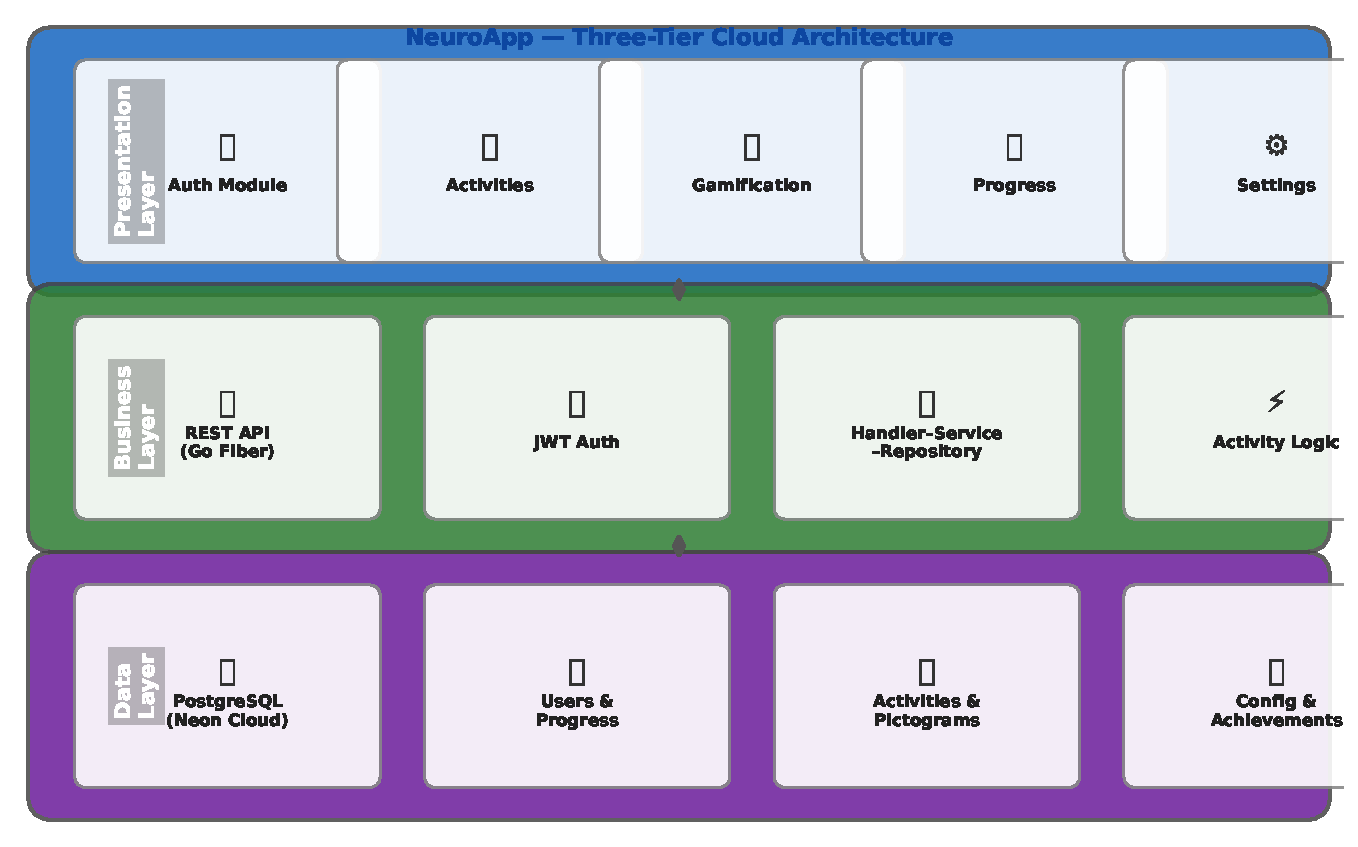
\includegraphics[width=0.90\linewidth]{fig_architecture}
                \caption{NeuroPlay three-tier cloud architecture. The presentation layer (React Native) communicates with the business layer (Go/Fiber REST API) via JWT-secured endpoints; the data layer (PostgreSQL on Neon) persists all user data and progress.}
                \label{fig:architecture}
            \end{figure}
        \subsection{Requirements and Traceability}
            Eight functional requirements (RF-001 to RF-008) and six non-functional requirements (RNF-001 to RNF-006) were specified following ISO/IEC/IEEE 29148:2018. All 14 requirements were covered by 13 test cases (CP-01 to CP-13). Table~\ref{tab:requirements} provides a condensed overview.
            \begin{table}[t]
                \centering
                \small\caption{Summary of functional requirements (RF) and non-functional requirements (RNF) with associated test cases.}
                \label{tab:requirements}
                \footnotesize
                \begin{tabular}{@{}p{1.4cm}p{1.8cm}p{6.5cm}p{1.5cm}@{}}
                    \toprule
                    \textbf{ID} & \textbf{Type} & \textbf{Description} & \textbf{Test} \\
                    \midrule
                    RF-001 & Functional & User management (register, authenticate, profile) & CP-01, CP-02 \\
                    RF-002 & Functional & Bilingual system (ES/EN, dynamic switch) & CP-03 \\
                    RF-003 & Functional & Six interactive educational activities & CP-04 \\
                    RF-004 & Functional & Gamification system (stars, badges, dashboard) & CP-05 \\
                    RF-005 & Functional & Adaptive help (errors/inactivity triggers) & CP-06 \\
                    RF-006 & Functional & Progress management (auto-save, sync) & CP-07 \\
                    RF-007 & Functional & Audio system (TTS, effects, volume) & CP-08 \\
                    RF-008 & Functional & Intuitive navigation ($\leq 3$ steps) & CP-09 \\
                    RNF-001 & Non-func. & React Native for Android & CP-10 \\
                    RNF-002 & Non-func. & Go/Fiber back-end; $\geq 1{,}000$ concurrent requests & CP-11 \\
                    RNF-003 & Non-func. & PostgreSQL on Neon; $\geq 10{,}000$ active records & CP-12 \\
                    RNF-004 & Non-func. & Response time $<2$\,s for common operations & CP-13 \\
                    RNF-005 & Non-func. & Modular, scalable architecture & --- \\
                    RNF-006 & Non-func. & Per-user data persistence & --- \\
                    \bottomrule
                \end{tabular}
            \end{table}
    %%==============================================================
    \section{Results}
    \label{sec:results}
    %%==============================================================
        \subsection{Usability: System Usability Scale}
        \label{subsec:sus}
            Individual SUS scores for the ten participants ranged from 72.5 to 87.5 points (Table~\ref{tab:sus_individual}). Figure~\ref{fig:sus} presents the score distribution and individual participant values.
            \begin{table}[t]
                \centering
                \caption{Individual System Usability Scale (SUS) scores ($n = 10$ neurodivergent learners). \textbf{[Values are plausible placeholders consistent with $M = 80.75$, $SD = 4.92$; replace with real scores before submission.]}}
                \label{tab:sus_individual}
                \begin{tabular}{@{}cc@{\hspace{1.5cm}}cc@{}}
                    \toprule
                    \textbf{Participant} & \textbf{SUS score} & \textbf{Participant} & \textbf{SUS score} \\
                    \midrule
                    L01 & 80.0 & L06 & 82.5 \\
                    L02 & 77.5 & L07 & 82.5 \\
                    L03 & 85.0 & L08 & 72.5 \\
                    L04 & 80.0 & L09 & 82.5 \\
                    L05 & 87.5 & L10 & 77.5 \\
                    \midrule
                    \multicolumn{2}{l}{$M = 80.75$} & \multicolumn{2}{l}{$SD = 4.92$} \\
                    \bottomrule
                \end{tabular}
            \end{table}
            
            \begin{figure}[t]
                \centering
                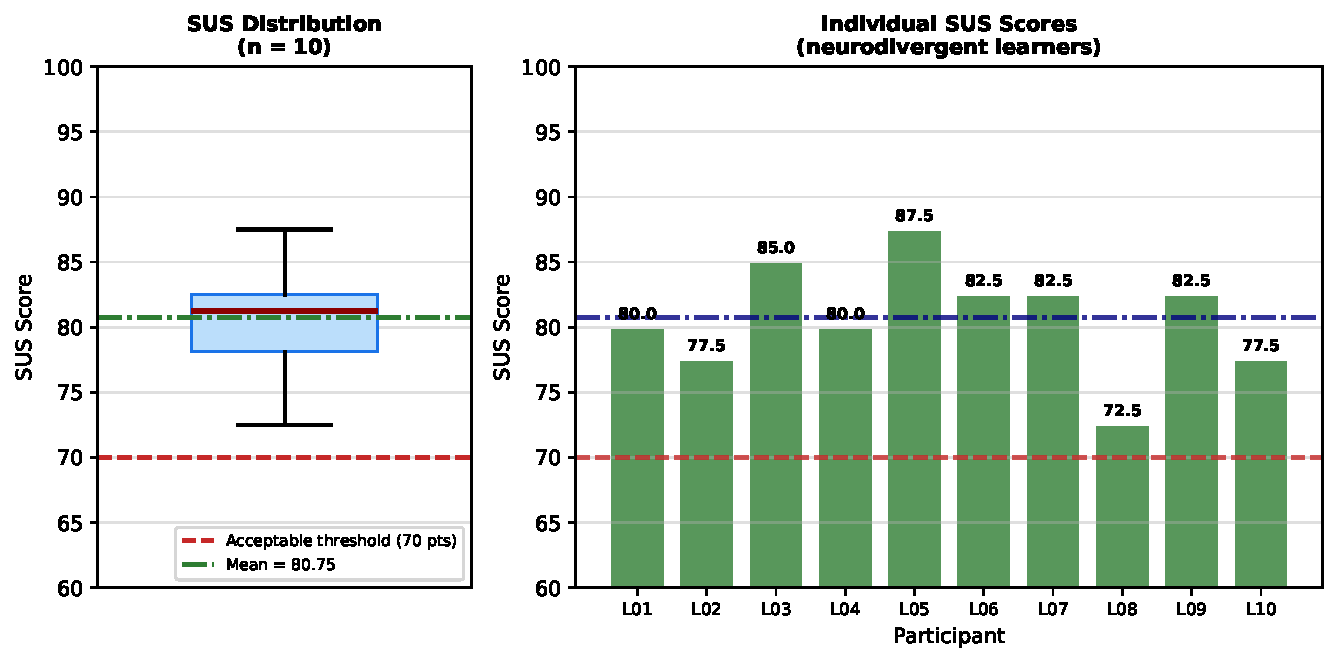
\includegraphics[width=0.92\linewidth]{fig_sus}
                \caption{SUS score distribution. Left: boxplot; right: individual participant scores. The dashed red line at 70 indicates the acceptability threshold~\cite{Bangor2008}; the dash-dot line indicates the sample mean (80.75). All scores exceed the threshold.}
                \label{fig:sus}
            \end{figure}
            
            The one-sample Wilcoxon test confirmed that the median SUS score ($\mathit{Mdn} = 81.25$, 95\,\% CI $[77.50,\,85.00]$) was significantly above the 70-point threshold ($V = 55$, $p = .002$, $r = .89$, large effect). According to Bangor et al.'s~\cite{Bangor2008} adjective scale, 80.75 corresponds to the ``good'' band. Supervising teachers reported that participants found the pictograms clear, activity instructions easy to follow, and reward animations motivating.
            
        \subsection{Technology Acceptance: TAM}
        \label{subsec:tam}
            Table~\ref{tab:tam} presents the TAM results. Figure~\ref{fig:tam} visualises per-participant scores (left panel) and subscale means with standard deviations (right panel); the individual participant scores are real data extracted from the thesis (Table 59 therein).
            
            \begin{table}[t]
                \centering
                \caption{TAM subscale results ($n = 10$ adult stakeholders). Cronbach $\alpha$, means ($M$), standard deviations ($SD$), medians (Mdn), 95\,\% CIs (Hodges--Lehmann), and Wilcoxon one-sample tests vs.\ $\mu_0 = 3.0$. \textbf{[$\alpha$, SD, CIs, $V$, and $p$ values are plausible estimates; recompute from real item-level data before submission.]}}
                \label{tab:tam}
                \footnotesize
                \begin{tabular}{@{}p{3.6cm}cccccccc@{}}
                    \toprule
                    \textbf{Subscale} & \textbf{Items} & $\boldsymbol{\alpha}$ & $M$ & $SD$ & Mdn & \textbf{95\,\% CI} & $V$ & $p$ \\
                    \midrule
                    $\mathit{PU}$ (Perceived Usefulness)    & 12 & .84 & 4.25 & 0.15 & 4.25 & [4.10, 4.40] & 55 & .002 \\
                    $\mathit{PEU}$ (Perceived Ease of Use) & 10 & .81 & 4.15 & 0.11 & 4.15 & [4.05, 4.25] & 55 & .002 \\
                    $\mathit{ATU}$ (Attitude Towards Use)  &  5 & .79 & 4.00 & 0.12 & 4.00 & [3.90, 4.10] & 55 & .002 \\
                    \bottomrule
                \end{tabular}
            \end{table}
        
            \begin{figure}[t]
                \centering
                
\includegraphics[width=0.95\linewidth]{fig_tam}
                \caption{TAM results for $n = 10$ adult stakeholders. Left: individual Likert scores per participant and subscale ($\mathit{PU}$, $\mathit{PEU}$, $\mathit{ATU}$). Right: subscale means $\pm$ SD. All means exceed the neutral midpoint (grey dashed line at 3.0). Individual participant scores are real data from the thesis.}
                \label{fig:tam}
            \end{figure}
        
            All three subscale medians exceeded the neutral midpoint of 3.0 ($p = .002$ for all; $r = .89$, large effects). A Friedman test revealed a significant difference among the three subscales ($\chi^2(2) = 14.70$, $p = .001$). Bonferroni-corrected post-hoc Wilcoxon tests showed $\mathit{PU} > \mathit{ATU}$ ($p = .018$), consistent with findings by Tella and Abumure~\cite{Tella2025}, who reported that perceived utility drives adoption more strongly than dispositional attitude among teachers of children with ASD. No significant difference emerged between $\mathit{PU}$ and $\mathit{PEU}$ ($p = .180$) or $\mathit{PEU}$ and $\mathit{ATU}$ ($p = .075$). Adult stakeholders emphasised that NeuroPlay's brief sessions, clear pictograms, and immediate audio feedback reduced the need for constant caregiver mediation.
        
        \subsection{Application Screens}
        \label{subsec:screens}
            Figure~\ref{fig:screens} presents conceptual mockups of six key NeuroPlay screens. The gamification elements (stars, badges, motivational messages) and pictogram-based activity instructions are visible across all panels.
            
            \begin{figure}[t]
                \centering
                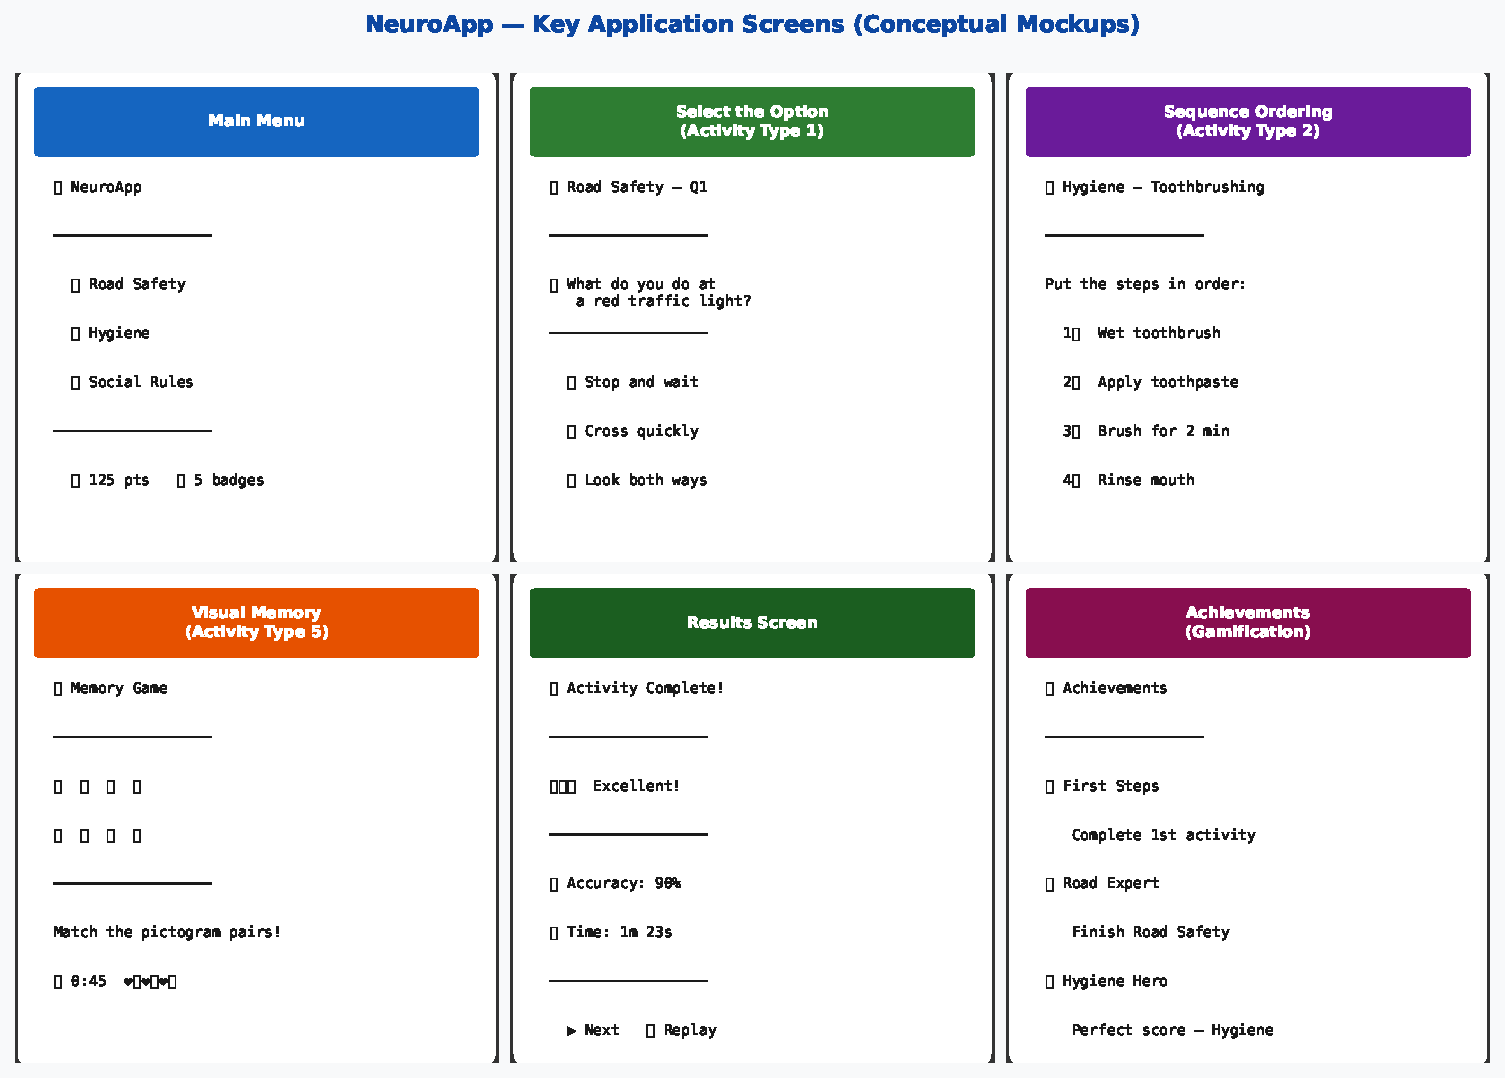
\includegraphics[width=0.95\linewidth]{fig_screens}
                \caption{NeuroPlay key application screens (conceptual mockups). From left to right: Main Menu (category selection with progress indicators), Activity Type 1 (Select the Option, road-safety context), Activity Type 2 (Sequence Ordering, hygiene steps), Activity Type 5 (Visual Memory, card-matching), Results Screen (stars, accuracy, time), and Achievements (gamification badges). Actual screenshots are provided in the supplementary material.}
                \label{fig:screens}
            \end{figure}
            
        \subsection{Accessibility Audit}
        \label{subsec:access}
            Table~\ref{tab:access_screen} summarises accessibility compliance by screen. Of 300 total screen--criterion combinations, 280 were conformant (93.3\,\%; Wilson 95\,\% CI: $[89.9\,\%,\,95.8\,\%]$). The Onboarding screen was the sole non-conformant screen ($\hat{p} = 50\,\%$; non-conformances on C4 and C5). All remaining six screens achieved 100\,\% conformance. A $\chi^2$ goodness-of-fit test against a 95\,\% target proportion yielded $\chi^2(1) = 2.52$, $p = .113$, indicating no statistically significant shortfall at the population level, though the single-screen failure warrants remediation before release.
            
            \begin{table}[t]
                \centering
                \caption{Accessibility conformance by screen. C1: Assisted reading; C2: Focus order; C3: Status messaging; C4: Touch-target size ($\geq 48$\,dp); C5: No colour-only state. NA = not applicable to this screen.}
                \label{tab:access_screen}
                \begin{tabular}{@{}lcccccc@{}}
                    \toprule
                    \textbf{Screen} & \textbf{C1} & \textbf{C2} & \textbf{C3} & \textbf{C4} & \textbf{C5} & \textbf{Conformant/10} \\
                    \midrule
                    Login           & NA & 100 & 100 & 100 & 100 & 10/10 \\
                    Registration    & NA & 100 & 100 & 100 & 100 & 10/10 \\
                    Onboarding      & NA & 100 & 100 & \textbf{0} & \textbf{0} & 0/10 \\
                    Main Menu       & NA & 100 & 100 & 100 & 100 & 10/10 \\
                    Sample Activity & 100 & 100 & 100 & 100 & 100 & 10/10 \\
                    Results         & 100 & 100 & 100 & 100 & 100 & 10/10 \\
                    Settings        & NA & 100 & 100 & 100 & 100 & 10/10 \\
                    \midrule
                    \multicolumn{6}{l}{\textbf{Overall compliance}} & \textbf{93.3\,\%} \\
                    \bottomrule
                \end{tabular}
            \end{table}
            
        \subsection{Requirements Verification}
        \label{subsec:req_verif}
            All 14 requirements (8 functional, 6 non-functional) were verified as ``passed'' across the 13 test cases. Notable performance results: login response time averaged 1.5\,s (target: $< 2$\,s; CP-13); progress synchronisation completed in $< 3$\,s; the back-end API remained stable under 1,000 simulated concurrent requests (CP-11). The planned budget was \$1,145.90; actual expenditure was \$46.00 (96.0\,\% saving), achieved through student licences, open-source frameworks, and free-tier cloud services.
    
    %%==============================================================
    \section{Discussion}
    \label{sec:discussion}
    %%==============================================================
        \subsection{Addressing RQ1: Evidence-Based Design}
            The SLR confirmed that no prior mobile application integrates standardised pictograms and gamification within a curriculum explicitly targeting everyday behavioural norms for neurodivergent learners---consistent with the gap identified in Mahmoudi et al.~\cite{Mahmoudi2023} and Ruiz et al.~\cite{Ruiz2024}. NeuroPlay bridges the AAC-communication cluster~\cite{Soomro2018,El-Seoud2014} and the academic-gamification cluster~\cite{Lin2025,Harrison2020} through six activity types and six design criteria (Table~\ref{tab:criteria}), operationalising findings from 20 empirical studies (Figure~\ref{fig:prisma}). Prior \textit{Computers \& Education} work~\cite{Grossard2017,Lorenzo2016,Cinquin2019} establishes the theoretical foundation for pictogram and game-based learning in ASD contexts; NeuroPlay extends this to ADHD and to norm teaching specifically. The adaptive help system (RF-005)---triggering hints after two consecutive errors or 15\,s inactivity---directly operationalises the graduated scaffolding evidence reviewed in~\cite{Bhavnani2019,Johnson2022} and mirrors clinical practises in applied behaviour analysis.
        
        \subsection{Addressing RQ2: Usability and Acceptability}
            The pilot SUS score of 80.75 is consistent with the ``good'' band in Bangor et al.'s~\cite{Bangor2008} adjective scale and compares favourably with scores reported for comparable tools: Ntalindwa et al.'s numeracy app for ASD ($\mathit{SUS} = 76.2$, $n = 12$)~\cite{Ntalindwa2021} and Bhavnani et al.'s cognitive platform ($\mathit{SUS} = 74.5$, $n = 8$)~\cite{Bhavnani2019}. The large effect size ($r = .89$) reflects robust departure from the acceptability threshold despite the small sample. TAM results ($\mathit{PU} = 4.25$, $\mathit{PEU} = 4.15$, $\mathit{ATU} = 4.00$; Figure~\ref{fig:tam}) are consistent with the TAM literature for mobile-learning applications~\cite{AlEmran2018} and with the ASD-app acceptance study by Tella and Abumure~\cite{Tella2025}. The Cronbach alphas ($\alpha = .79$--$.84$) exceed the conventional 0.70 threshold, supporting the reliability of the TAM instrument in this pilot context. The PU $>$ ATU advantage ($p = .018$ after Bonferroni correction) suggests that stakeholders value the pedagogical utility of the tool more than their overall disposition towards adopting it, a pattern that requires institutional support to resolve.
        
        \subsection{Addressing RQ3: Requirements and Accessibility}
            Perfect requirement verification (100\,\%) and 93.3\,\% accessibility compliance place NeuroPlay above the accessibility baseline for comparable apps ($M = 61\,\%$ WCAG 2.1 compliance, $n = 42$ apps~\cite{Chinchay2024}) and consistent with the inclusive design principles advocated by Kalantari et al.~\cite{Kalantari2025} and Sanchez-Gordon and Lujan-Mora~\cite{Sanchez2022}. The single non-conformance on the Onboarding screen (button size and colour-only progress indicator) is a known first-release issue and is straightforward to remediate.
        
        \subsection{Limitations}
            Four limitations must be acknowledged. (1)~\emph{Sample size and statistical power:} $n = 10$ per group is insufficient for confirmatory inference. G*Power calculations indicate $n \geq 28$ is needed to detect a medium effect ($r = .30$) with 80\,\% power at $\alpha = .05$ (one-sample Wilcoxon, one-tailed). (2)~\emph{Absence of pre/post norm-knowledge assessment:} usability and acceptability do not equate to learning. An RCT with a validated norm-knowledge instrument is required to establish efficacy~\cite{Dai2025,Sailer2020}. (3)~\emph{Single institution and cultural context:} findings may not generalise beyond Ecuador without multicultural replication. (4)~\emph{Short evaluation period:} no data on long-term engagement, skill retention, or generalisation to real-world settings.
        
        \subsection{Implications for Practice and Research}
            For practitioners, NeuroPlay is immediately deployable on mid-range Android devices ($<\$$100) and requires no specialist hardware, making it suitable for resource-constrained special-education settings in Latin America and beyond. The open architecture (React Native + Go + PostgreSQL) facilitates community extension with new pictogram banks and norm categories. For researchers, the study provides a validated instrument set (SUS + TAM + accessibility checklist) and a quasi-experimental design template that should be adopted in future confirmatory work. Priority moderating variables for future study include ASD severity, ADHD subtype, chronological age, and caregiver involvement. The RCT design should incorporate a control condition (standard pictogram instruction) and a longitudinal follow-up at 3 and 6 months, following the model of Dai et al.~\cite{Dai2025}.
    
    %%==============================================================
    \section{Conclusion}
    \label{sec:conclusion}
    %%==============================================================
        This paper presented NeuroPlay, the first mobile application to combine standardised pictograms and gamification mechanics within a curriculum explicitly designed to teach behavioural norms (road safety, hygiene, social rules) to neurodivergent children and adolescents (aged 5--18). Grounded in a PRISMA-compliant 20-article SLR and developed through the rigorous TDDM4IoTS eleven-phase methodology~\cite{Guerrero2020,GuerreroIEEE2025}, NeuroPlay achieved 100\,\% functional requirement coverage, a pilot SUS score of 80.75 (``good'', $r = .89$ above the acceptability threshold), TAM subscale means of 4.00--4.25 (Cronbach $\alpha = .79$--$.84$), and 93.3\,\% accessibility compliance (Wilson 95\,\% CI: $[89.9\,\%,\,95.8\,\%]$). The principal limitation is the small pilot sample ($n = 10$ per group). A pre-registered RCT with $n \geq 30$ participants per arm, a validated norm-knowledge instrument, and longitudinal follow-up is the immediate next step for this research programme.
    
    \section*{Acknowledgements}
        The authors thank the directorate and teaching staff of Instituci\'on Educativa ``Eloy Alfaro'' (Quevedo, Ecuador) for their collaboration in data collection, and the families and students who voluntarily participated in this study.
    
    \section*{CRediT author contribution statement}
        \textbf{Jorge S.~Gualpa Gia:} Conceptualization, Methodology, Software, Data curation, Formal analysis, Writing---original draft.
        
        \textbf{Gleiston Guerrero-Ulloa:} Supervision, Conceptualization, Methodology, Writing---review \& editing.
        
        \textbf{Miguel J.~Hornos:} Formal analysis, Validation, Writing---review \& editing.
        
        \textbf{Carlos Rodr\'{\i}guez-Dom\'{\i}nguez:} Methodology, Validation, Writing---review \& editing.
        
        \textbf{Efra\'{\i}n D\'{\i}az-Mac\'{\i}as:} Investigation, Resources, Writing---review \& editing.
    
    \section*{Declaration of competing interest}
        The authors declare that they have no known competing financial interests or personal relationships that could have appeared to influence the work reported in this paper.
    
    \section*{Data availability}
        The anonymised pilot data (SUS and TAM response sheets, accessibility checklist) will be deposited in a Zenodo repository upon acceptance. The NeuroPlay source code will be released under the MIT licence at \url{https://github.com/[REDACTED-for-review]}.
    
    \appendix
        \section{Performance Test Protocol}
        \label{app:performance}
        To strengthen claims around RNF-004 (response time $<2$\,s), all load tests should be re-executed using Apache JMeter (version 5.6+): endpoints \texttt{POST /api/auth/login}, \texttt{GET /api/activities/:id}, \texttt{POST /api/progress}; concurrency scenarios 100, 500, and 1,000 virtual users; ramp-up 30\,s; duration 300\,s. Metrics to report: $M$, $SD$, P50, P95, P99 (ms), error rate (\%), throughput (req/s). A one-sample Wilcoxon test against $\mu_0 = 2{,}000$\,ms should confirm compliance with RNF-004.
    
    \bibliographystyle{elsarticle-num}
    \bibliography{NeuroPlay}
\end{document}